% !TEX program = xelatex

\documentclass{outline-of-mechanics}

\begin{document}
%\widowpenalty0
%\clubpenalty0

% 封面
\includepdf{body/F00-Frontpage.pdf}
\bookmark[page=1,level=0]{封面}

% 标题页
\includepdf{body/F01-Titlepage.pdf}
\bookmark[page=2,level=0]{封页}

% 出版信息页
\documentclass[../outline-of-mechanics.tex]{subfiles}

\begin{document}
% 出版信息页
\begin{center}
  \zihao{4}\fangsong\mbox{}

  \mbox{}\label{publish}\pdfbookmark{出版页}{publish}

  责任编辑:张晓红

  封面设计:陈治黄

  \vfill \heiti{力~~学~~概~~论}

  \normalsize \kaishu{方励之~~李淑娴}

  \normalfont{} *

  安徽科学技术出版社出版

  \zihao{-5} (合肥市跃进路1号)

  \normalsize 安徽省%
  \hspace{0.2em}\raisebox{-0.5mm}{\includegraphics[width=4em]{icon/xinhuabokestore}}\hspace{0.2em}%
  发行~~安徽新华印刷厂印刷

  *

  \zihao{6}开本:850$\times$1168~~1/32~~印张:12.5~~字数:309,000

  1986年1月第一版~~~~1986年1月第一次印刷

  印数00,001—5,000

  \normalsize 统一书号:13200$\cdot$68~~~~定价:2.50元
\end{center}
\thispagestyle{empty}
\clearpage
\end{document}


% 内容提要
\documentclass[../outline-of-mechanics.tex]{subfiles}

\begin{document}
% 内容提要
\begin{center}
  \begin{minipage}{8.4cm}\vspace{3cm}
    \label{abstract}\pdfbookmark{内容提要}{abstract}
    \begin{center}\heiti{内\quad 容\quad 提\quad 要}\end{center}
    \zihao{-5}
    \hspace{2em}本书是根据作者在中国科学技术大学及北京大学讲授普通物理的
    力学部分讲稿整理而成的。其特点是强调用物理的前沿发展去改进基础物理教
    学,即用现代物理的观点去选择课程的内容,去表现概念和规律。因此,书中
    包括一些在传统的教材中没有的内容,如牛顿宇宙学等,对许多传统的内容,
    也采取新的讲授法,使之能与当代物理的进展相呼应。另外。由于力学是物理
    学的入门和基础,所以本书也注意物理方法的阐述,这对于初学物理的学生是
    有益的。书中还附有一些习题及答案。

    \hspace{2em}本书可作为综合大学及师范院校的普通物理力学教材,也可供大
    专院校物理教师及物理教学研究工作者参考。
  \end{minipage}
\end{center}
\thispagestyle{empty}
\clearpage
\end{document}


% 序言
\documentclass[../outline-of-mechanics.tex]{subfiles}

\begin{document}
\setcounter{page}{1}
\pagestyle{foreword}
\null\vspace{1em}
\begin{center}
  \label{foreword}\pdfbookmark{序}{foreword}
  \zihao{4}\heiti{序}

  \null{}
\end{center}
\fangsong\normalsize

这本书原是一份普通物理课程的力学讲义,它曾在中国科学
技术大学沿用多年,也曾在北京大学教授过数次。

普通物理中的力学,是相当难教的,凡是教授过这门课的老
师,大都有此体会。一方面,力学是整个物理学的基石,它包含
许多基本的观念、方法和理论,需要学生极为准确地加以掌握,
以备后继学习之用,另一方面,初入大学的学生,往往看轻力学,
误认为新的内容不多,似乎在中学里都已学过,结果力学反而被
疏忽了。

这种局面迫使一些教师采用理论力学的方法来教授普通物理
力学。这样做,确实可以解决前述问题的第二方面,学生不再感
到“似曾相识”了。随着教和学二者的提高,原属理论力学的部
分内容的确可以逐渐放到普通物理中来。但是,我们觉得,若仅
限于这一途径改进教学,还不能或不完全能解决问题的第一个方
面——力学是整个物理的一块基石。

基石到底在哪里起了基石的作用?基石到底如何起了基石的
作用?显然,这些“哪里”,这些“如何”只有从物理的当代发
展以及前沿研究的角度,才能看得清楚。这就是说,如果我们企图
从“物理的基石”这一标准来组织教学,它至少有以下两方面的
含义:一是不断用新的现代的观点去整理老的内容,一是不断用新
的前沿的重要成果来充实基础。事实上,不同时代的教材的差别,
最清楚地表现在这些方面。上述的标准,也就是我们在编写这本
教材时,尝试着去追求的。也许有的地方达到了,也许有的地方%分页处
并未达到。无论成功或失败,它都是我们的追求的记录。

为了使用上的方便,书中编辑了一些例题,每章末也附有一
些思考题和习题。由于北京大学物理系和中国科学技术大学物理
教研室已编有《物理学习题集》(人民教育出版社,1980),为了不
重复太多,本书中的例题和习题只是标志性的。在教学上需要更
多习题时,可以参考上述的习题集。

在使讲义变成这本书的过程中,得到过员汝槐同志的协助,
谨致谢意。

\null{}

\hspace{6.8cm}\zihao{-4}\kaishu{作~~~者}

\mbox{}

\hspace{7cm}\normalfont{} \zihao{-5}1984年4月\normalsize
\clearpage
\end{document}


% 目录
\clearpage
\setcounter{page}{1}
\pdfbookmark{目录}{Contents}
\tableofcontents

% 正文
\clearpage
\pagestyle{heading}
\setcounter{page}{1}
\setcounter{chapter}{-1}
% 公式与上下文本距离调整
%\baselineskip=1.5em
\lineskip=0.25em
\lineskiplimit=0.25em
\abovedisplayskip=0.25em plus 0.25em minus 0.25em
\belowdisplayskip=\abovedisplayskip
\abovedisplayshortskip=0em plus 0.25em minus 0.25em
\belowdisplayshortskip=\abovedisplayshortskip
\belowcaptionskip=-0.8em
%\def\int{\mathop{\vcenter{\hbox{\scaleto[1.3ex]{\symbol{"222B}}{2em}}}}\nolimits}
%\def\sum{\mathop{\vcenter{\hbox{\scaleto{\symbol{"2211}}{1.2em}}}}}

% 绪论
\documentclass[../outline-of-mechanics.tex]{subfiles}

\begin{document}

\ctexset{chapter={number={\symbol{"3000}},name={绪,论}}}
\chapter[物理世界的统一]{—— ~ 物理世界的统一}\label{chp:0}
\ctexset{chapter={number={\chinese{chapter}},name={第,章}}}

物理学的兴起,是从经典力学开始的。在经典力学之前,人类
的文明中虽然已有不少具有物理价值的发现和发明,但是并不存
在一门独立的物理学。因此,我们在学习经典力学的时候,首先
应当了解:为什么经典力学成了物理学的起点?经典力学在整个
物理学中占据着怎样的地位?

爱因斯坦曾经这样来概括牛顿力学的历史地位;“古代希腊
伟大的唯物主义者坚持主张,一切物质事件都应当归结为一系列
的有规律的原子运动,而不允许把任何生物的意志作为独立的原
因。而且无疑笛卡尔曾按他自己的方式重新探索过这一问题。但
是,在当时,它始终不过是一个大胆的奢望,一个哲学学派的成
问题的理想而已。在牛顿之前,还没有什么实际的结果来支持那
种认为物理因果关系有完整链条的信念。”

这句话的意思是,物理学依赖于一种基本的信念:物理世界
存在着完整的因果链条,即自然界是统一的。牛顿力学则是体现
这种信念的第一个成功的范例。

从牛顿力学的创建到现在,已经有三百多年了,物理学已经
大大发展了,远远超过了经典力学原有的水平。但是,就物理学
的最基本的追求和物理学的总目标来说,却一直没有变化。经典
力学时代的追求和目标,可以说时至今日仍然是整个物理学的追
求和目标。这个最基本的追求和目标,就是自然界的统一。的确,
从整个物理学的发展中,可以看到一条鲜明的主线。这就是执着%分页点
地追求宇宙的统一,找寻支配宇宙万物的最基本最统一的规律。

相信存在统一,努力寻求统一,如果仅仅作为一种自然观,
早在古代已经有了。老子的《道德经》中写有:“道生一、一生
二、二生三、三生万物。”这就是中国古代的一种统一观,它完
全可以与爱因斯坦所提及的古希腊的哲学相媲美。不过,无论在
古代中国或古希腊,统一观都只是一种哲学思辨。

牛顿的力学和古代的哲学不同,它不是思辨地坚持统一观,
而是发展了寻找统一的有效的物理方法。牛顿在他的最重要的力
学著作《自然哲学的数学原理》中阐明了他采用的方法。他在前
言中写道;“我奉献这一作品。作为哲学的数学原理,因为哲学
的全部责任似乎在于——从运动的现象去研究自然界中的力,然
后从这些力去说明其他的现象。”\sbfootnote{牛顿这段话里的
  “哲学”一词,实际含义相当于今天的“科学”或“物理学”。}这就是
说,寻求统一的出发点不是思辨而应是运动现象。自然界中的运动
现象是多种多样的,物理学的责任就在于寻找支配这些现象的统一的力。

今天的物理学,仍然大体地沿袭着牛顿所开创的研究途径。
寻找统一的力,或统一的相互作用。因此,几乎所有基本的物理
理论都称做某种力学,如牛顿力学、电动力学、色动力学等等。
每一种新的力学的确立,都标志着我们在追求统一的逾程上达到
了一个新的水平。

为了更具体地表达上述的论述。我们利用表1。表1左边列举
的是自然界中的种种运动现象,也就是物理学的研究对象。天体
的运行和地面物体的运动是人首先看到或接触到的,随后才有时
间、空间的概念,所以时空也是一种物理研究的对象,另一类现
象是电、磁和光,所有这些物理对象。在二十世纪之前,人们都
已知道了。二十世纪以来,又逐渐证实或发现一些新的对象。如
原子、原子核、核子以及夸克等。

\clearpage
表\ref{tab:00.01}~的其余部分就表示物理学在寻求统一,寻求完整的因果
链条上一些重要的阶段。
牛顿的力学和万有引力定律,是物理学上第一次大的统一。
在牛顿之前,传统的观念认为支配天体运行和支配地面物体运动
的规律是不相同的,有所谓天界和世俗两个世界之分。然而,牛
顿发现,天上行星和月亮的运动,实际上和地面落体运动遵从相
同的规律,它们都是由引力引起的。这样,牛顿就用他的力学打
破了天界和世俗的界限,找到了两个世界的统一。牛顿称引力为
万有引力,就是强调这种统一。

第二次大的统一,是由十九世纪的麦克斯韦完成的。他建立
了电磁理论,使电、磁及光学现象得到统一。这就是电动力学。

很快发现,牛顿的力学和麦克斯韦的电磁学这两大领域在时
\begin{table}[!h]
  \centering
  \caption{物理学发展中的统一$^*$}\label{tab:00.01}
  \begin{tabular}{c}
    \toprule \vspace{-1em}            \\
    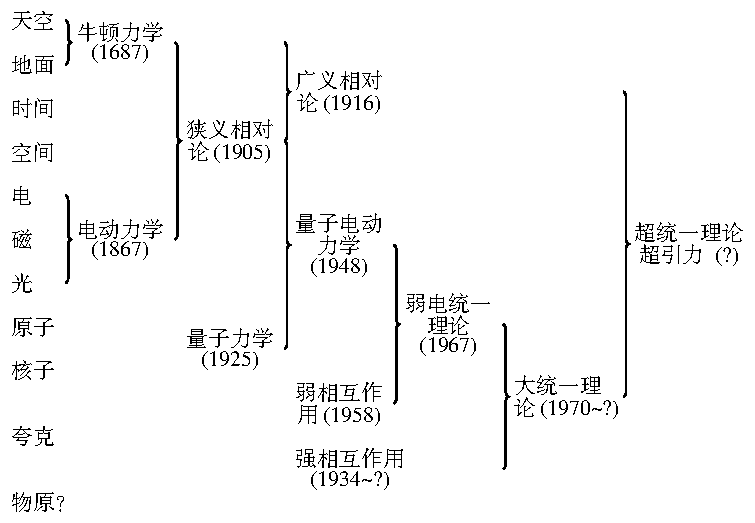
\includegraphics[scale=0.76]{figure/tab00.01} \\
    \bottomrule
    \zihao{6}* 括号中的数字表示相应的理论建立的年代;有问号的表示尚未完成。
  \end{tabular}
\end{table}
\clearpage\noindent 空观上是很不协调的。在前者中,各种匀速运动是平权的,但却
假定有绝对空间或绝对速度存在。相反,在后者中,有一个地位
特殊的速度,即光速,但却始终测不出这个特殊的速度是相对于
哪一个绝对空间而言的。爱因斯坦抛弃了绝对空间观念,使电磁
学、力学在新的时空观的基础上达到了协调和统一。

爱因斯坦还曾企图把引力和电磁力二者统一起来,但他的努
力没有成功。然而,他却找到了能与麦克斯韦电磁理论相协调的
引力理论——广义相对论。

作为引力理论的广义相对论和作为电磁理论的麦克斯韦理论
构成了我们今天称为经典物理学的理论基础。

与经典物理相对的是量子论。量子力学最初是作为原子、分
子的统一的力学而发展起来的。这种新的力学统一地解释了原子、
分子的各种光谱现象,统一地解释了元素周期表,统一地解释了
各种不同分子的键合。

在将量子力学扩展到电磁场时,遇到了困难,这本质上是由
于电磁场是相对论性的。直到四十年代末,发展了所谓重整化方
法才巧妙地解决了上述的困难,使量子论与电磁理论能得以统一,
产生了量子电动力学。

到六十年代末,我们已经得到了如下的物理世界的图象。宇
宙中的所有物理对象可以分成两大类,一类称为“物质”,如夸
克、电子、$\mu$子等等,另一类称为“相互作用”,如引力、电磁力
等等。在目前的宇宙中,有四种基本的相互作用,按它们的强度
顺序排列是:核子参与的强相互作用,荷电粒子参与的电磁相互
作用,核子及电子、中微子参与的弱相互作用,以及任何粒子都
参与的引力相互作用。可以简单地说,宇宙间的一切运动和变化。
都可以统一为这四种“力”的作用。但是,追求统一的物理学,
似乎认为这种状况仍然不够统一。

1967年,温伯格和萨拉姆再次着眼于统一,先后提出了电磁
相互作用和弱相互作用的统一理论。随后的一系列实验证明他们
的统一理论是正确的。

这一新的成功,促使许多人去找寻把电磁作用、弱作用及强
作用都包含在内的统一理论,通常称为“大统一理论”。建立这
种理论的工作还没有完成,这是正在研究的领域。

如果大统一能够顺利完成,下一步的统一就是要把引力也统
一在内了。引力是物理学最早讨论的一种基本的力。但是,它与
其他力的统一最难,因为引力有一系列很特别的性质。例如这种
力只有引力却无斥力。就是这种特别性质之一。

企图把引力与其他力统一起来的工作,称为超统一的研究。
目前还没有得到有实际意义的结果。它是今天的物理学的一个前
沿。实现超统一的一个可能是用超引力理论,这种理论中的统一
有一个很有趣的特点,即它把物理学中传统的“物质”与“相互
作用”之间的界限也打破了。

总之,从牛顿力学开始,物理学就在寻找宇宙的统一,我们
希望找到控制着万事万物运动的极少的几个基点。只有从这个角
度我们才容易看清经典力学在整个物理学中的地位和作用,也才
能全面地了解学习经典力学对于学习整个物理学的意义和作用。

\end{document}

% 第一章
\documentclass[../outline-of-mechanics.tex]{subfiles}

\begin{document}

\chapter{时间,空间和运动学}\label{chp:01}

\subfile{M01.01-Time}
\subfile{M01.02-Zeno Paradox And Measurement Of Time}
\subfile{M01.03-Length}
\subfile{M01.04-Reference Frame}
\subfile{M01.05-Trajectory}
\subfile{M01.06-Instantaneity Of Velocity}
\subfile{M01.07-Velocity Of Curvilinear Motion}
\subfile{M01.08-Acceleration}
\subfile{M01.09-Circular Motion And Angular Velocity}
\subfile{M01.10-Uniform Circular Motion}
\subfile{M01.11-Inverse Problem In Kinematics}
\subfile{M01.12-Consider Questions}
\subfile{M01.13-Exercises}

\end{document}


% 第二章
\documentclass[../outline-of-mechanics.tex]{subfiles}

\begin{document}

\chapter{运动学中的相对性}\label{chp:02}

\subfile{M02.01-Relative And Absolute}
\subfile{M02.02-Relativity Of Position And Trajectory}
\subfile{M02.03-Relativity Of Velocity}
\subfile{M02.04-Relativity Of Acceleration}
\subfile{M02.05-Galileo Transformation}
\subfile{M02.06-Failure Of Velocity Composition Law}
\subfile{M02.07-The Conclusions Of Invariance Of Light Velocity 1 - Time Dilation}
\subfile{M02.08-The Conclusions Of Invariance Of Light Velocity 2 - Length Contraction}
\subfile{M02.09-Consider Questions}
\subfile{M02.10-Exercises}


\end{document}


% 第三章
\documentclass[../outline-of-mechanics.tex]{subfiles}

\begin{document}

\chapter{牛顿动力学}\label{chp:03}

\subfile{M03.01-Inertia Law}
\subfile{M03.02-Newton's Second Law}
\subfile{M03.03-Newton's Third Law}
\subfile{M03.04-Some Specific Forces}
\subfile{M03.05-Some Simple Applications Of Newtonian Mechanics}
\subfile{M03.06-Consider Questions}
\subfile{M03.07-Exercises}

\end{document}


% 第四章
\documentclass[../outline-of-mechanics.tex]{subfiles}

\begin{document}

\chapter[万有引力]{\makebox[5em][s]{万有引力}}\label{chp:04}

\subfile{M04.01-Kepler's Three Laws Of Planetary Motion}
\subfile{M04.02-The Establishment Of The Law Of Gravitation}
\subfile{M04.03-Gravitational Constant G}
\subfile{M04.04-Unit System And Dimension}
\subfile{M04.05-Several Important Gravitational Physical Quantities}
\subfile{M04.06-Geometry Of Force}
\subfile{M04.07-Gravitational Action In Multi-Particle System}
\subfile{M04.08-Consider Questions}
\subfile{M04.09-Exercises}

\end{document}


% 第五章
\documentclass[../outline-of-mechanics.tex]{subfiles}

\begin{document}

\chapter[牛顿宇宙学]{牛顿宇宙学}\label{chp:05}

\subfile{M05.01-The Copernican Principle}
\subfile{M05.02-Cosmic Density Distribution}
\subfile{M05.03-Several Velocity Distribution Solutions}
\subfile{M05.04-Oberst Paradox And Cosmic Expansion}
\subfile{M05.05-Cosmic Expansion Dynamics}
\subfile{M05.06-Consider Questions}
\subfile{M05.07-Exercises}

\end{document}


% 第六章
\documentclass[../outline-of-mechanics.tex]{subfiles}

\begin{document}

\chapter[能量守恒]{\makebox[5em][s]{能量守恒}}\label{chp:06}

\subfile{M06.01-Conservation Of Mechanical Energy}
\subfile{M06.02-Work}
\subfile{M06.03-Gravitational Potential Energy}
\subfile{M06.04-Conservative Force}
\subfile{M06.05-General Properties Of One-Dimensional Motion}
\subfile{M06.06-Consider Questions}
\subfile{M06.07-Exercises}

\end{document}


% 第七章
\documentclass[../outline-of-mechanics.tex]{subfiles}

\begin{document}

\chapter[振动]{\makebox[5em][s]{振动}}\label{chp:7}

\subfile{M07.01-Elastic Force}
\subfile{M07.02-Vibration Solution}
\subfile{M07.03-Geometric Expression Of Simple Harmonic Vibration}
\subfile{M07.04-Damped Vibration And Q Value}
\subfile{M07.05-Resonance}
\subfile{M07.06-Simple Harmonic Vibration Synthesis}
\subfile{M07.07-Consider Questions}
\subfile{M07.08-Exercises}

\end{document}


% 第八章
\documentclass[../outline-of-mechanics.tex]{subfiles}

\begin{document}

\chapter[动量守恒]{\makebox[5em][s]{动量守恒}}\label{chp:08}

\subfile{M08.01-Conservation of Momentum}
\subfile{M08.02-Impulse}
\subfile{M08.03-Collision}
\subfile{M08.04-Center Of Mass Theorem}
\subfile{M08.05-Consider Questions}
\subfile{M08.06-Exercises}

\end{document}


% 第九章
\documentclass[../outline-of-mechanics.tex]{subfiles}

\begin{document}

\chapter{角动量守恒}\label{chp:09}

\subfile{M09.01-Conservation of Angular Momentum.tex}
\subfile{M09.02-Moment}
\subfile{M09.03-Lung-Lenz vector}
\subfile{M09.04-Moment of Inertiar}
\subfile{M09.05-Kinetic Energy of Rotation}
\subfile{M09.06-Consider Questions}
\subfile{M09.07-Exercises}

\end{document}


% 第十章
\documentclass[../outline-of-mechanics.tex]{subfiles}

\begin{document}

\chapter[刚体]{\makebox[5em][s]{刚体}}\label{chp:10}

\subfile{M10.01-Degrees of Freedom and Degrees of Freedom of Rigid Body}
\subfile{M10.02-Translation and Rotation}
\subfile{M10.03-Kinetic Energy of Rigid Body}
\subfile{M10.04-Rigid Body Equations of Motion}
\subfile{M10.05-Gyro}
\subfile{M10.06-Cosider Question}
\subfile{M10.07-Exercises}

\end{document}


% 第十一章
\documentclass[../outline-of-mechanics.tex]{subfiles}

\begin{document}

\chapter{狭义相对论基础}\label{chp:11}

\subfile{M11.01-Pragmatic Inertial Reference Frame}
\subfile{M11.02-Principle of Relativity}
\subfile{M11.03-Basic Principle of Special Relativity}
\subfile{M11.04-Lorentz Transform}
\subfile{M11.05-Space-Time Idea of Relativity}
\subfile{M11.06-Mechanics of Relativity}
\subfile{M11.07-Mass-Energy Relation}
\subfile{M11.08-Cosider Question}
\subfile{M11.09-Exercises}

\end{document}


% 第十二章
\documentclass[../outline-of-mechanics.tex]{subfiles}

\begin{document}

\chapter{动力学与非惯性参考系}\label{chp:12}

\subfile{M12.01-Non-Inertial Reference Frame and Inertial Force}
\subfile{M12.02-Rotation Reference Frame}
\subfile{M12.03-Criticism of Absolute Space-Time}
\subfile{M12.04-Equivalence Principle}
\subfile{M12.05-Local Inertial Frame}
\subfile{M12.06-Cosider Question}
\subfile{M12.07-Exercises}

\end{document}


% 习题答案
\documentclass[../outline-of-mechanics.tex]{subfiles}



\begin{document}
\clearpage
\pagestyle{plain}
\refstepcounter{chapter}
\chapter*{全部习题答案}
\addcontentsline{toc}{chapter}{全部习题答案}
\setlength{\mathindent}{4em}
\setcounter{chapter}{0}
\setcounter{figure}{0}
\newcounter{answer}

\renewcommand{\figurename}{答案图}

\newcommand{\achapter}{
  \setcounter{answer}{0}
  \setcounter{figure}{0}
  \addtocounter{chapter}{1}
  \begin{center}
    \textsf{第\chinese{chapter}章}
  \end{center}
}

\newlength{\itemwidth}
\settowidth{\itemwidth}{88.}
\setlength{\parindent}{1.75em}
\newcommand{\answer}{
  \noindent
  \addtocounter{answer}{1}
  \makebox[\itemwidth][l]{\theanswer .}
}

\newlength{\xindent}
\settowidth{\xindent}{(2) }
\newcommand{\aindent}{\makebox[\xindent]{}}

\subfile{M13.01-Answers-Chp01}
\subfile{M13.02-Answers-Chp02}
\subfile{M13.03-Answers-Chp03}
\subfile{M13.04-Answers-Chp04}
\subfile{M13.05-Answers-Chp05}
\subfile{M13.06-Answers-Chp06}
\subfile{M13.07-Answers-Chp07}
\subfile{M13.08-Answers-Chp08}
\subfile{M13.09-Answers-Chp09}
\subfile{M13.10-Answers-Chp10}
\subfile{M13.11-Answers-Chp11}
\subfile{M13.12-Answers-Chp12}

\end{document}


% 重排后记
\documentclass[../outline-of-mechanics.tex]{subfiles}


\begin{document}
\clearpage
\pagestyle{empty}
\setcounter{page}{1}
\label{afterword}\pdfbookmark{重排后记}{afterword}
\begin{center}
  \zihao{3}\xbsong 重\hspace{0.333em}排\hspace{0.333em}后\hspace{0.333em}记
\end{center}
\vspace{1em}

《力学概论》,方励之、李淑娴合著,安徽科学技术出版社出版。1986年1月第一次出版。

作者自述道:“这本书原是一份普通物理课程的力学讲义,它曾在中国科学
技术大学沿用多年,也曾在北京大学教授过数次。”实际上,即使在某事件
之后学校改用梁昆淼先生的《力学》作为正式教科书,也在相当长的一段时间
内作为实际的教科书在科大学子和老师中沿用。

由于某些原因,该书已经不可能再出版了,纸质书籍也难以觅得踪迹。网上仅
见一份1986年1月第一版的扫描本,精度较差,字迹模糊,不少细节难以
分辨。本重排版采用\LaTeX 根据该扫描本重新编排并绘制了
全部插图(个别图片替换为网上寻得的高清晰图片),对明显的错漏做了更正。

由于原书铅字人工排版印刷,与\LaTeX 排版相比,存在较大差异。在重排过
程中,无法实现完全相同的效果,只能在可能的情况下,尽量按照原书页码安排内容。

重排版全部源代码文件在网上公开,项目地址如下:
\begin{center}
  \href{https://github.com/chianjin/outline-of-mechanics}{https://github.com/chianjin/outline-of-mechanics}
\end{center}

当然个人精力、水平有限,亦难免遗漏或者改错之处。阅读者如有发现,可
前往上述网址讨论或提交相关信息。如有兴趣者,亦可在上述项目网址联系
本人参与修订。

\clearpage
\label{tips}\pdfbookmark{特别提示}{tips}
\heiti \zihao{4}
\begin{center}
  ~\\
  特\hspace{0.333em}别\hspace{0.333em}提\hspace{0.333em}示
\end{center}
\normalsize
\vspace{1em}

该书的版权、著作权由原作者、出版机构及该书权利人所有。如需商用,请与原作者、出版机构及该书权利人联系。

~

本重排版仅作个人学习之用。若有侵犯原书相关权利人权利,请联系本人删除网络发布。
\thispagestyle{empty}

\end{document}


% 重排校注
%\clearpage{\pagestyle{empty}\cleardoublepage}
%\input{body/Z02-Errata Note}

\end{document}
